\documentclass[10pt,a4paper]{article}
\usepackage[utf8]{inputenc}
\usepackage[italian]{babel}
\usepackage{amsmath}
\usepackage{amsfonts}
\usepackage{amssymb}
\usepackage{siunitx}
\usepackage{graphicx}
\usepackage[left=2cm,right=2cm,top=2cm,bottom=2cm]{geometry}
\newcommand{\rem}[1]{[\emph{#1}]}
\graphicspath{ {../Figs-Tabs/} } % graphics search directories

\author{Gruppo BF \\ Andrea Luzio, Gianfranco Cordella, Valerio Lomanto}
\title{Esercitazione N.1: Misure di tensione, corrente, tempi, frequenza.}
\begin{document}

\maketitle

\section{Scopo e strumentazione}

L'esercitazione ha lo scopo di verificare la risposta in frequenza dei filtri passivi. Si misurano le caratteristiche principali di tali circuiti come guadagno in tensione e frequenze di taglio.

\section{Filtro passa-basso}
\paragraph{2.a }
Abbiamo montato il circuito in Fig. 1 con i valori di resistenza e capacità misurati con il multimetro digitale: $R_1 = 816\pm 7 \Omega$ , $R_2 = 99.7\pm 0.9 k\Omega$ e $C_1 = 110\pm 5 nF$. L'errore è stato stimato usando le indicazioni del manuale del multimetro.La frequenza di taglio attesa è $f_\mathrm{t}= \frac{1}{2\pi R_1C_1}= 1.77 \pm 0.09 kHz $.
Utilizzando l'oscilloscopio si sono misurati i rapporti tra le ampiezze della tensione in entrata e ai capi del condensatore a due frequenze diverse.
L'attenuazione intorno ai $2 kHz$ misurata è di $-3.4 dB$ contro un valore atteso di $-3.6 dB$. A $20 kHz$ si ha un valore atteso di $-21 dB$ contro una misura di $-20 dB$. 

\paragraph{2.b}
\'E stata misurata la frequenza di taglio (usando il frequenzimetro dell'oscilloscopio) come la frequenza compatibile ocn un'attenuazione di $-3dB$; essa risulta essere $f_t =1.88 \pm 0.05 kHz$. L'errore è stato stimato vedendo per quale variazione di frequenza si apprezza una variazione di ampiezza sull'oscilloscopio.
Si è inoltre misurata la suddetta frequenza di taglio con un fit a due rette(fit affine delle code $f<100 Hz$ e $f>14 kHz$  ) e con un fit della funzione di attenuazione (guadagno in $dB$). 
Si possono vedere i fit in \ref{f:fit1}. 
\begin{figure}
	\centering
	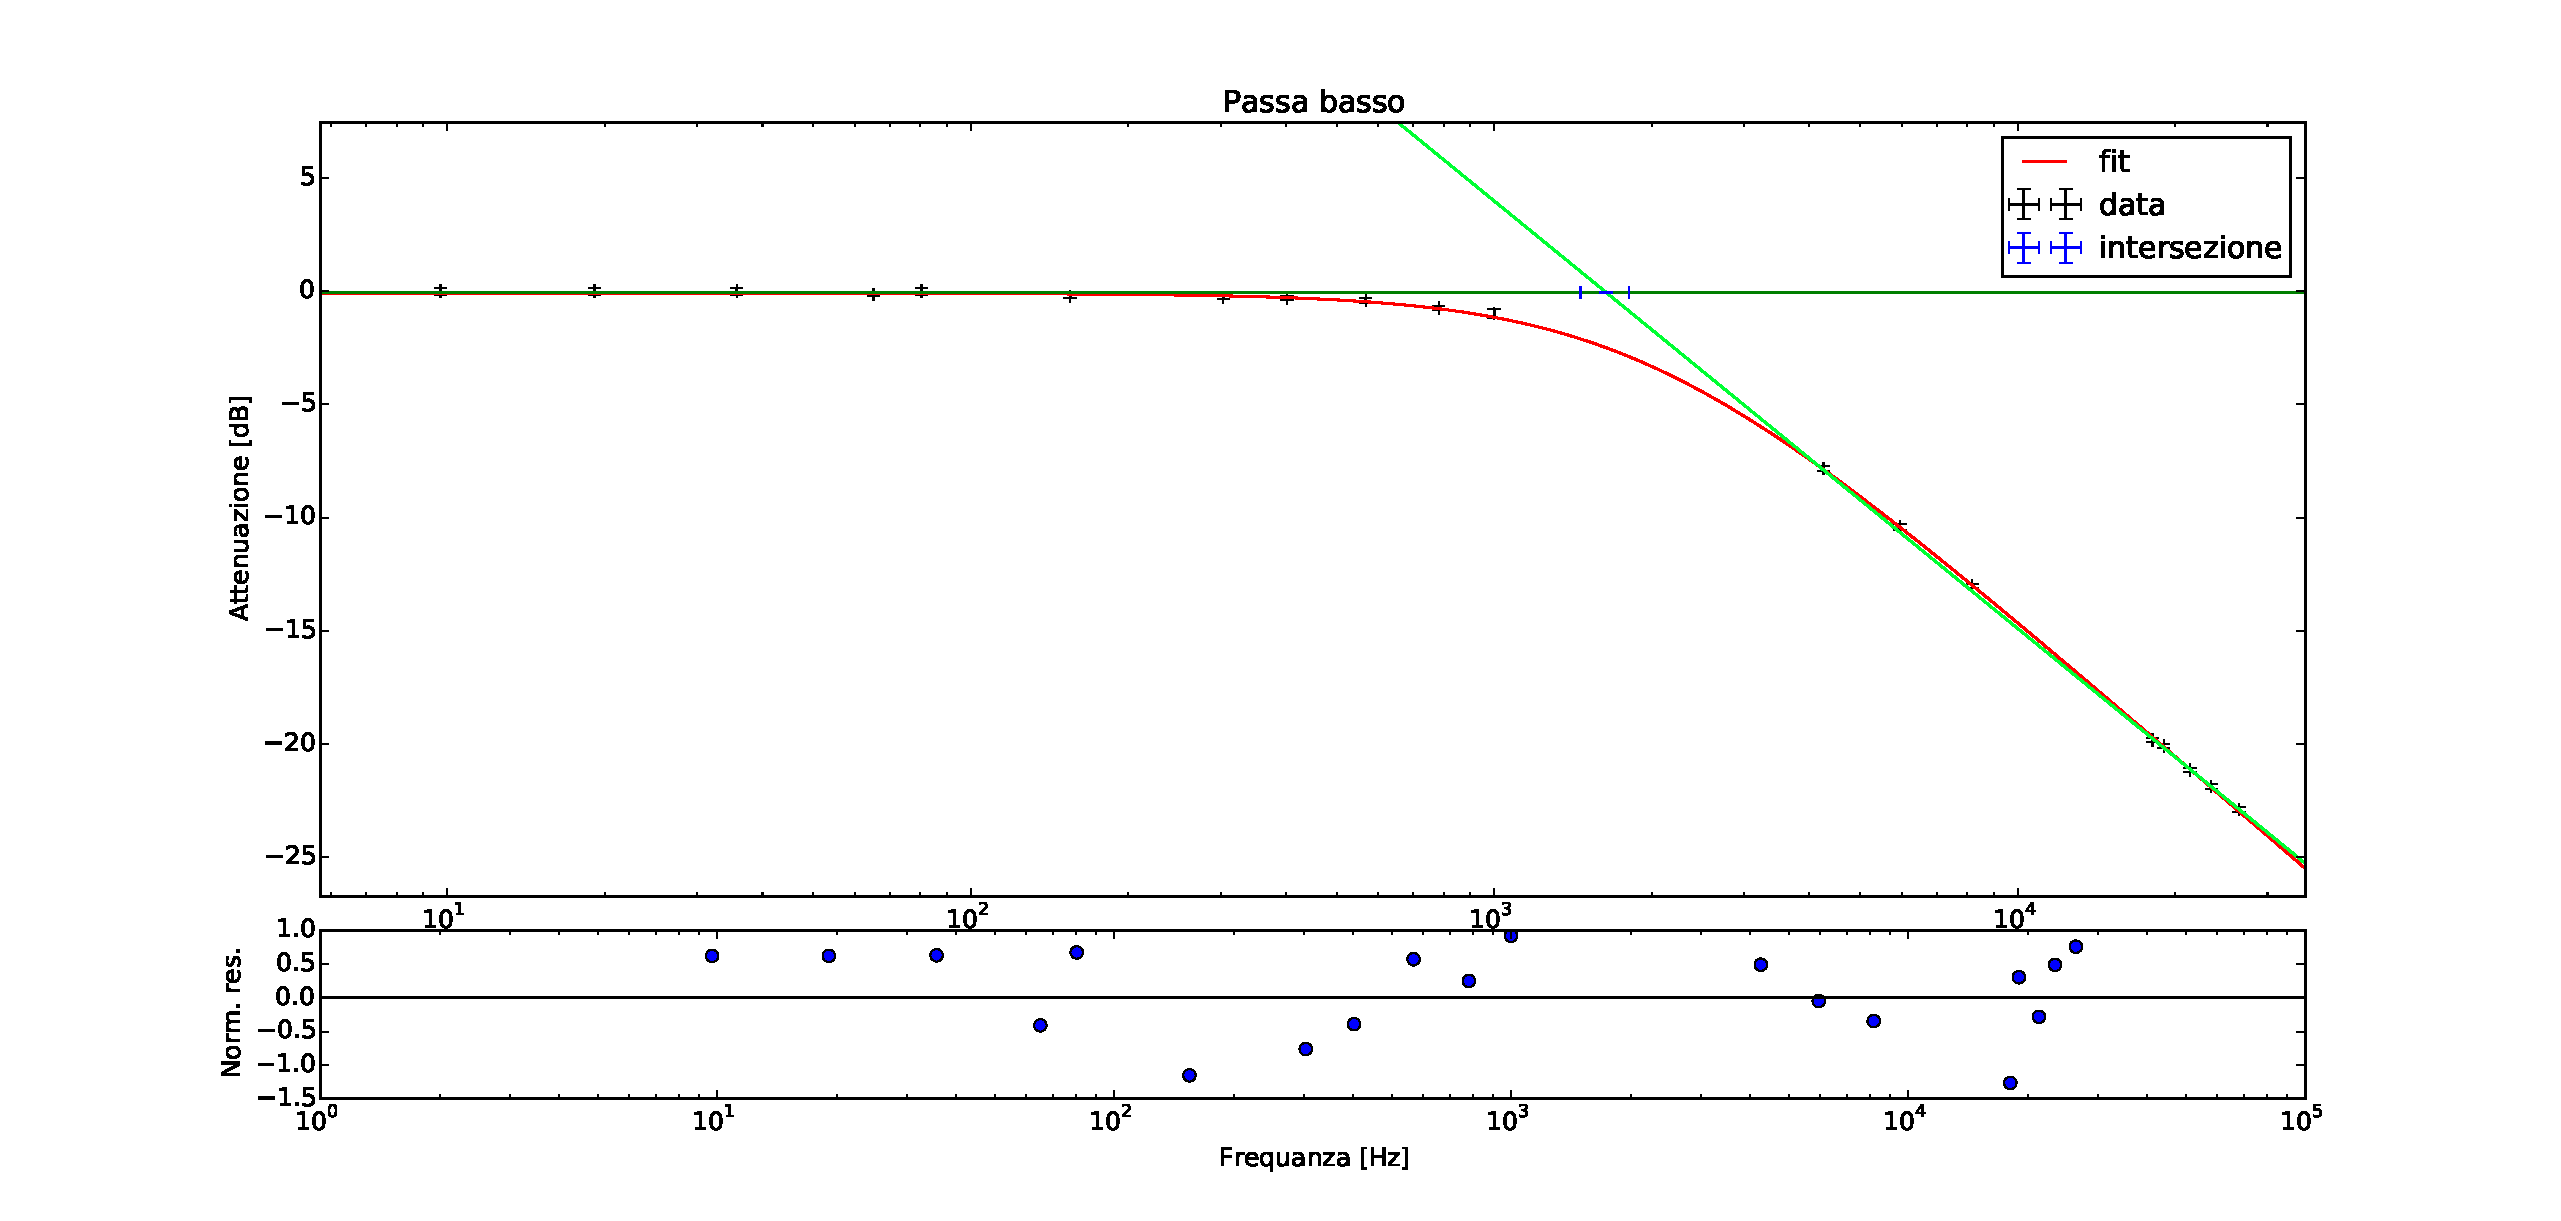
\includegraphics[scale=0.4]{plt_passa_basso.pdf}
	\caption{Grafico di Bode e fit trasferimento del passa-basso.\label{f:fit1}}
\end{figure}

I parametri trovati sono rispettivamente:\\
$f_t=1.64\pm 0.17 kHz$ e $f_t=1.90 \pm 0.01 kHz$. Nel fit dell'attenuazione si è ottenuto un $\chi^2=8 (/17 dof)$.
Si può notare che in alta frequenza la retta fittata ha una pendenza di $-18.9\pm 0.8 dB/decade$. Questo ci può suggerire che un possibile problema sia una sottostima della frequenza alla quale si può approssimare la funzione di trasferimento con la sua retta asintotica.

Il risultato trovato non è in perfetto accordo con il valore calcolato sulla base delle caratteristiche dei componenti scelti. Non ci sentiamo comunque di garantire una completa non compatibilità.


\paragraph{3 risposta al gradino }
Si è generata un'onda quadra e si è misurato il tempo di salita ,della tensione ai capi dell'oscilloscopio, usando i cursori dell'oscilloscopio. Il tempo di salita misurato è : $t_salita = 192 \pm 4 \mu s$.
Da cui si ricava $f_t = 1.82 \pm 0.04 kHz $. La misura è compatibile con il valore atteso di $1.77 \pm 0.09 kHz $.

\paragraph{4  }
L'impedenza di ingresso di un filtro passa-basso è : $Z_in = R_1 + \frac{f_t}{jf} $. A basse frequenze $Z_in$ diverge a infinito mentre ad alte frequenze il circuito è puramente resistivo.Per $f=f_t$ risulta invece $Z_in = R_1(1-j)$. 
La resistenza di carico in generale altera il funzionamento del circuito iniziale. Tuttavia se tale resistenza è molto maggiore della serie tra $R_1 e C_1$ allora la tensione all'uscita del condensatore viene completamente trasferita al carico stesso. Questa situazione rispecchia quella ideale in cui l'inserimento di un componente non altera il funzionamento del circuito iniziale. Perciò se abbasso la resistenza del carico a $10 k\Omega$, la differenza percentuale  $\frac{V_{out}(R_L)-V_{out}}{V_{out}} = \frac{R_1/R_L}{(V_{out})^4}$ risulta del $32 \%$ alla frequenza di taglio del circuito iniziale contro un valore del $3 \%$ per $R_L=100 k\Omega$.

\begin{figure}
	\centering
	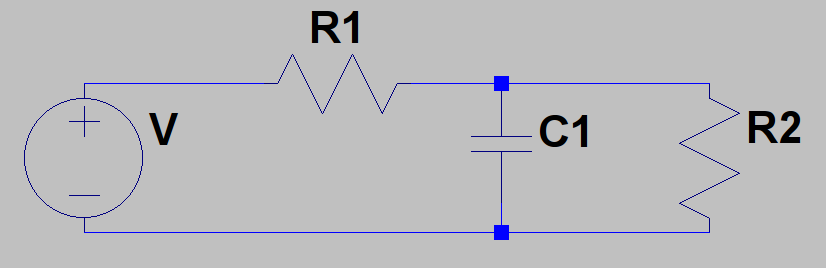
\includegraphics[scale=0.4]{passa_basso.png}
	\caption{Filtro passa-basso (con carico).\label{f:p-basso}}
\end{figure}


\section{Filtro passa-banda}
\paragraph{Filtro RC passa-basso}
Si è montato il circuito passa-basso come in Figura (\ref{f:p-basso}) (misurando l'uscita sul condensatore ) con $R_1= 3.22 \pm 0.04 k\Omega $ e $C_1= 10.7 \pm 0.4 nF $ . Si è verificato che l'andamento del guadagno fosse quello previsto, cioè pari a 1 per $f << f_t$ e tendente a zero per $f>> f_t$. Si è misurato un guadagno di $-3 dB$ ad una frequenza di $4.7 \pm 0.1 kHz$  che è compatibile con quello attesa di $4.6 \pm 0.2 kHz$.

\paragraph{Filtro RC passa-alto}
Si è montato il circuito passa-alto (misurando l'uscita sulla resistenza)con $R= 3.28 \pm 0.04 k\Omega $ e $C_1= 110 \pm 4 nF $ . Si è verificato che l'andamento del guadagno fosse quello previsto, cioè pari a 0 per $f << f_t$ e tendente 1 per $f>> f_t$. Si è misurato un guadagno di $-3 dB$ ad una frequenza di $461.6 \pm 0.1 Hz$  che è compatibile con quello atteso di $439 \pm 21 kHz$.
\paragraph{Filtro passa-banda}
Si è montato il circuito in Figura\ref{passa_banda} con i valori di resistenze e capacità già usate nei punti precedenti. Usando i cursori dell'oscilloscopio si sono misurate le ampiezze picco-picco della tensione in ingresso e di quella in uscita da $R_2$. La frequenza è stata misurata usando il frequenzimetro dell'oscilloscopio. Dal fit dei dati risulta che il guadagno di centro banda sia $-6.35 \pm 0.04 dB$. Le frequenze di taglio misurate attraverso le intersezioni delle rette fittate nelle tre regioni sono $f_h = 279 \pm 6 Hz $ e $f_l = 9.2 \pm 0.5 kHz$\footnote{$f_l$ è quella di taglio del passa-basso mentre $f_h$ è quella del passa-alto}; anche qua le pendenze troppo basse (17.5 e -18.8 dB/decade) suggeriscono che non abbiamo raggiunto con le frequenze controllate la zona asintotica. Il valore atteso del guadagno di centro banda ($-5.9 \pm 0.1$ dB) non è compatibile con quello ottenuto dal fit, presumibilmente poiché nella zona di frequenze comprese tra quelle di taglio non è mai possibile approssimare ad 1 entrambi i guadagni. I valori di $f_h$ e $f_l$ sono rispettivamente compatibili con il doppio e la metà di delle frequenze di taglio dei due circuiti separati.
Nel fit della funzione di attenuazione si è ottenuto, con un $\chi^2=14 (/24 dof)$, un valore di $458 \pm 3 Hz$ per la frequenza di taglio del passa-alto e di $4.95 \pm 0.03$ per quella del passa-basso, entrambe compatibili con quanto atteso.
Nel caso di $R_2 >> R_1$ si ottiene che la resistenza di ingresso del passa alto risulta molto maggiore di quella di uscita del passa basso quindi la tensione ai capi del condensatore $C_1$ viene completamente trasferita come ingresso del passa alto. Quindi la funzione di trasferimento risulta essere il prodotto delle due.

\begin{figure}
\centering
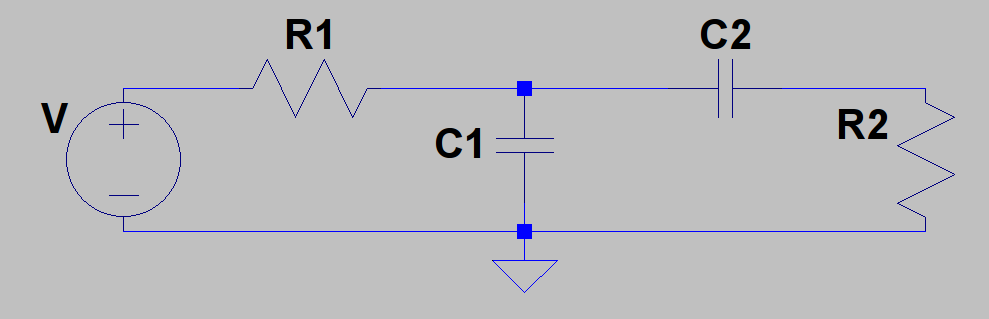
\includegraphics[scale=0.4]{passa_banda.png}
\caption{Filtro passa-banda.\label{passa_banda}}
\end{figure}

\begin{figure}
	\centering
	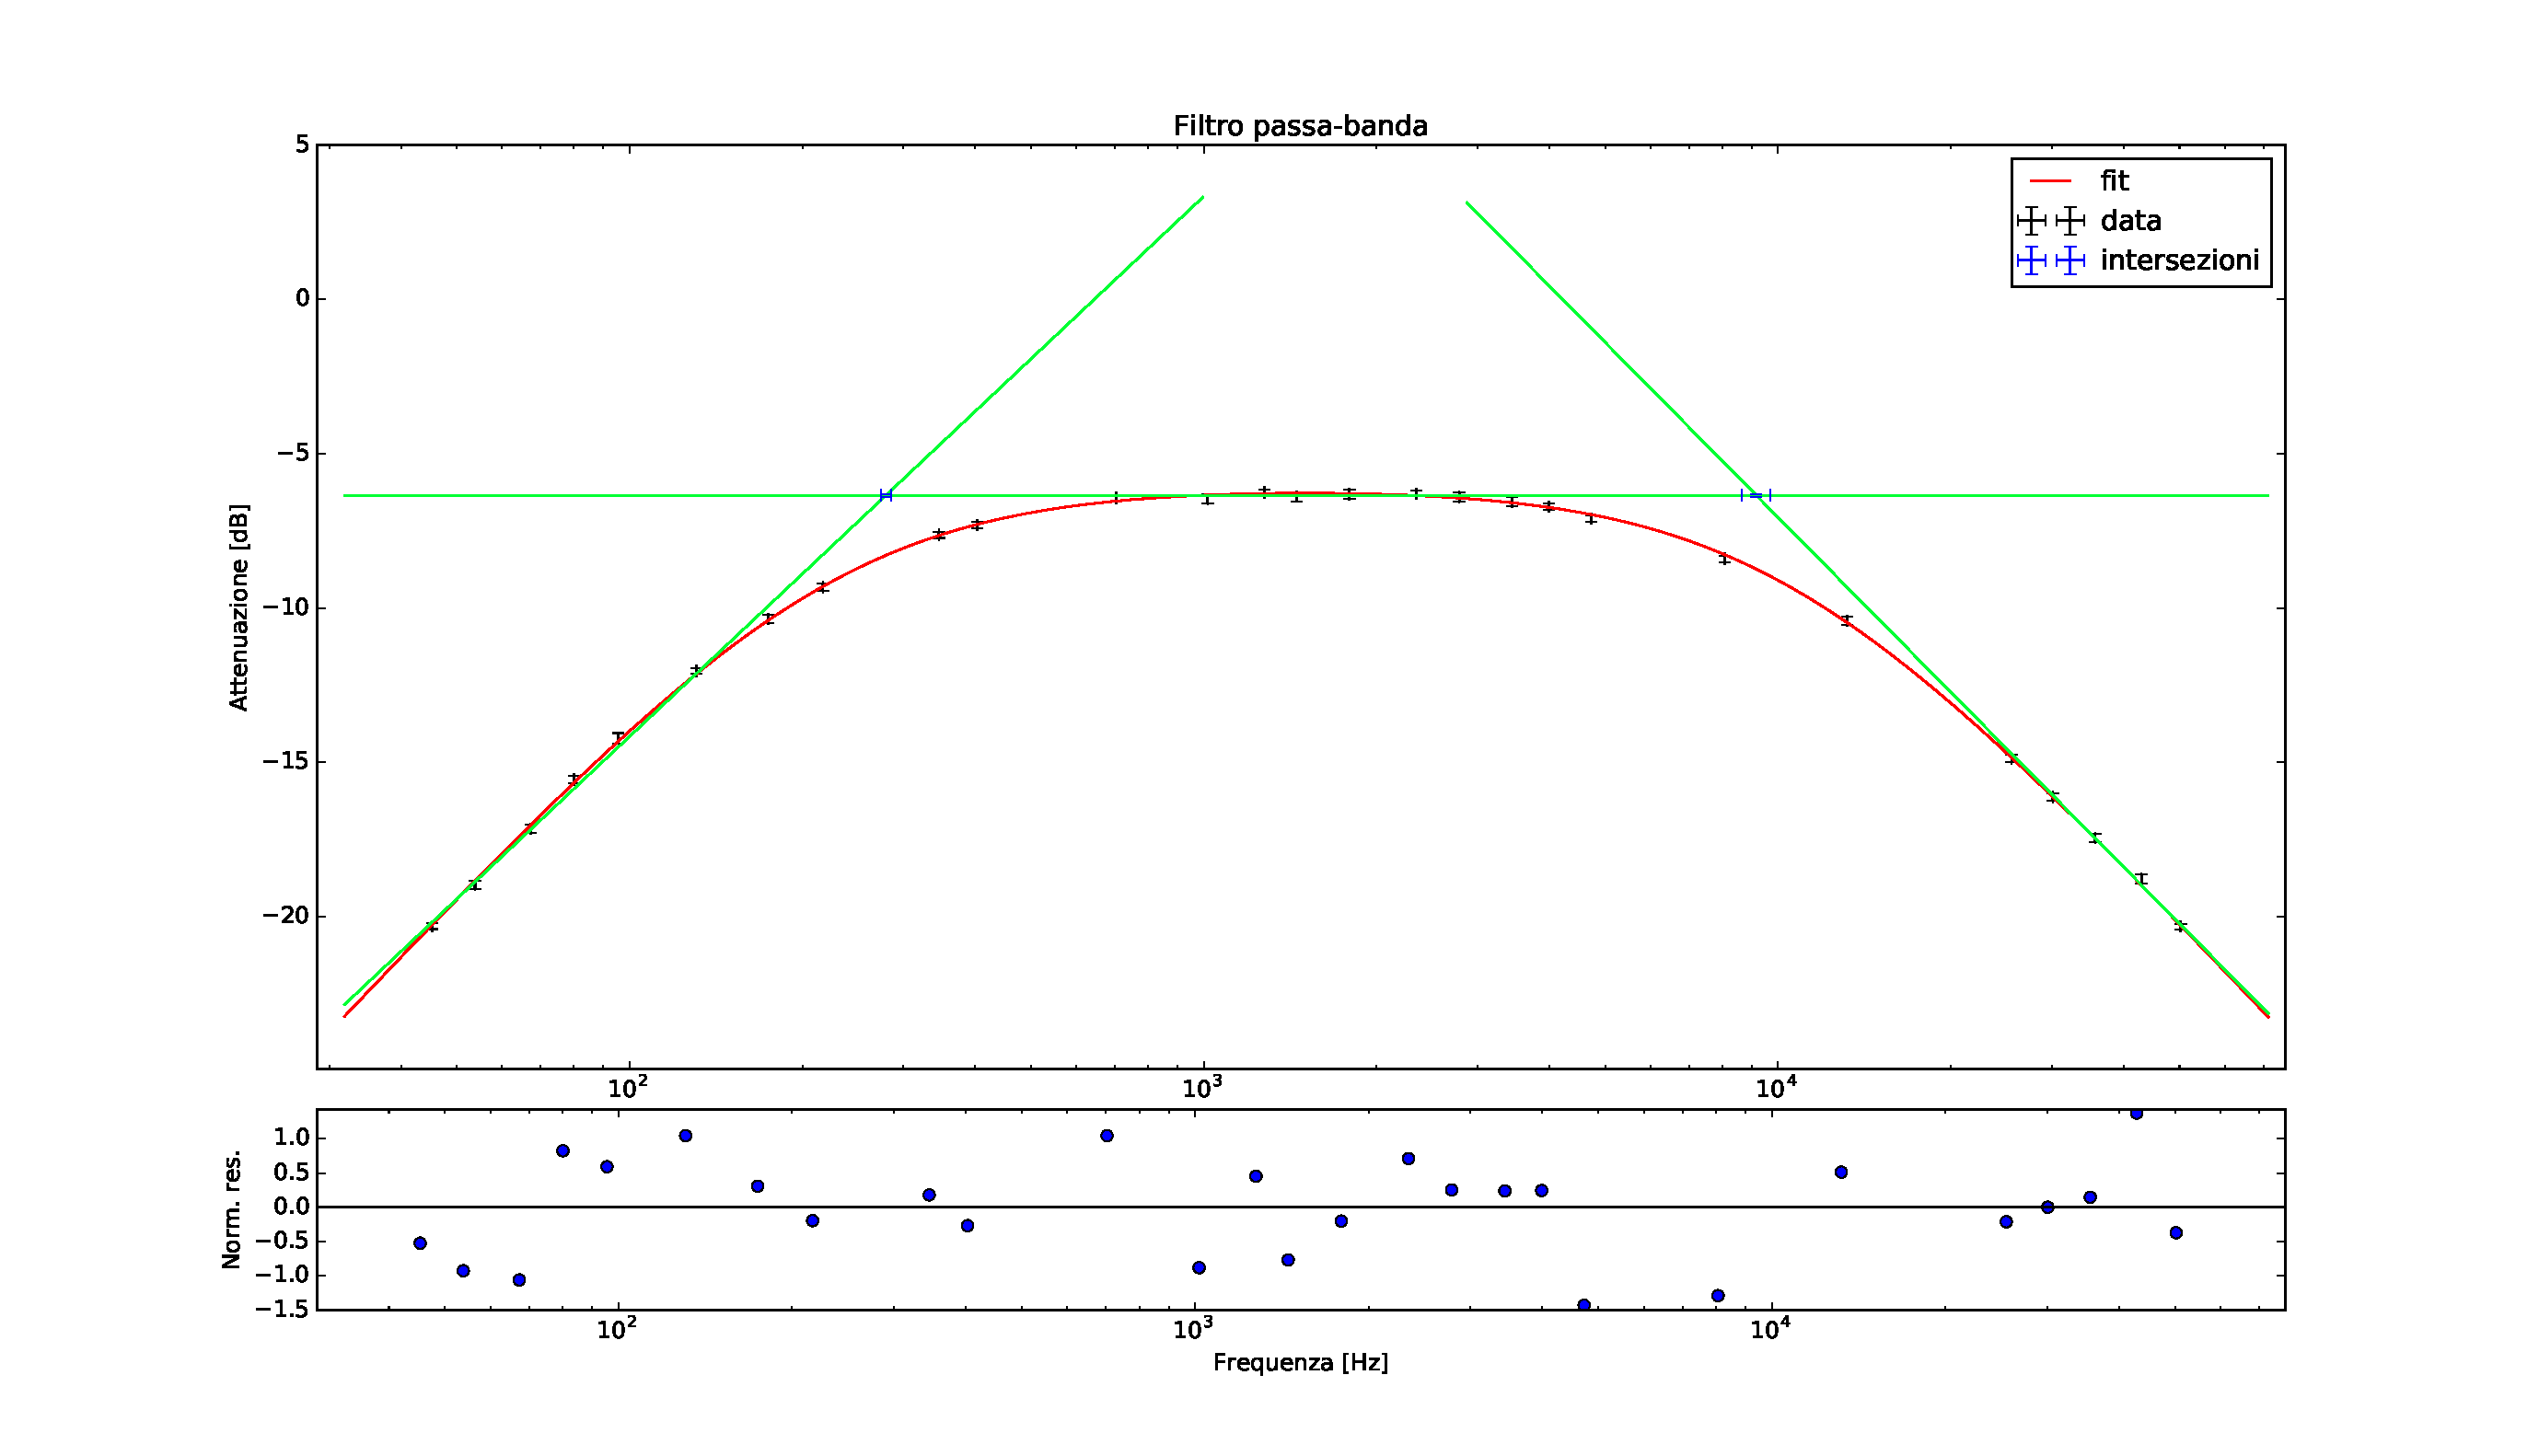
\includegraphics[scale=0.4]{plt_passa_banda.pdf}
	\caption{Grafico di Bode e fit trasferimento del passa-banda.\label{f:fit1}}
\end{figure}


\end{document}